%% LyX 2.2.1 created this file.  For more info, see http://www.lyx.org/.
%% Do not edit unless you really know what you are doing.
\documentclass[english]{article}
\usepackage[T1]{fontenc}
\usepackage[latin9]{inputenc}
\usepackage{geometry}
\geometry{verbose,tmargin=0.1\paperheight,bmargin=0.1\paperheight,lmargin=0.1\paperwidth,rmargin=0.1\paperwidth}
\usepackage{babel}
\usepackage{varioref}
\usepackage{url}
\usepackage{graphicx}

\makeatletter
%%%%%%%%%%%%%%%%%%%%%%%%%%%%%% User specified LaTeX commands.
\renewcommand{\partname}{Partie}

\@ifundefined{showcaptionsetup}{}{%
 \PassOptionsToPackage{caption=false}{subfig}}
\usepackage{subfig}
\makeatother

\usepackage{listings}
\renewcommand{\lstlistingname}{Listing}

\begin{document}

\title{Cellular Automata \\
(implemented in C)}

\author{Maxandre Jacqueline,\\
1st-Year SABS student}
\maketitle

\part{Motivation}
\begin{quotation}
``Three centuries ago science was transformed by the dramatic new
idea that rules based on mathematical equations could be used to describe
the natural world. My purpose {[}...{]} is to initiate another such
transformation, and to introduce a new kind of science that is based
on the much more general types of rules that can be embodied in simple
computer programs.'' Stephen Wolfram \cite{wolfram2002new}
\end{quotation}
Mathematicians traditionally use mathematical formulas to describe
reality, but Stephen Wolfram argues that it only makes sense when
the behaviour of the system under investigation is computationally
reducible.\cite{wolfram2002new} Traditional mathematics tries to
find shortcuts, or ``tricks'' as Richard Feynman once said, to describe
an observed system, so that computing predictions involves less computational
power than it took for the system to perform its behaviour.\cite{wolfram2002new}One
can neverless doubt that such tricks can be found for complex systems.
Traditional science has focused on reducing complex systems to its
elementary components so they can be tractable by mathematical tricks,
but missing at the same time the emergent behaviour of complex interacting
systems. For example, it is claimed biological systems are extremely
complex and have emergent properties that cannot be explained, or
even predicted, by studying their individual parts in isolation. \cite{van2004reductionism}
\begin{quotation}
``Models based on cellular automata provide an alternative approach
{[}to differential equations{]}. {[}...{]} They exhibit {[}analogous{]}
complicated behavior, but by virtue of simpler construction are potentially
amenable to a more detailed and complete analysis.'' Stephen Wolfram
\cite{wolfram1983statistical}
\end{quotation}
Some cellular automata (such as rule 30 cellular automaton, see figure
\vref{fig:The-rule-30}) exhibit a particularly interesting property
called ``intrinsic randomness generation''\cite{wolfram2002new}.
A system without random input can behave in what most would call random.
Stephen Wolfram argues that ``this is how much of the randomness
that we see in nature arises''.\cite{wolfram2002new}

\begin{figure}

\centerline{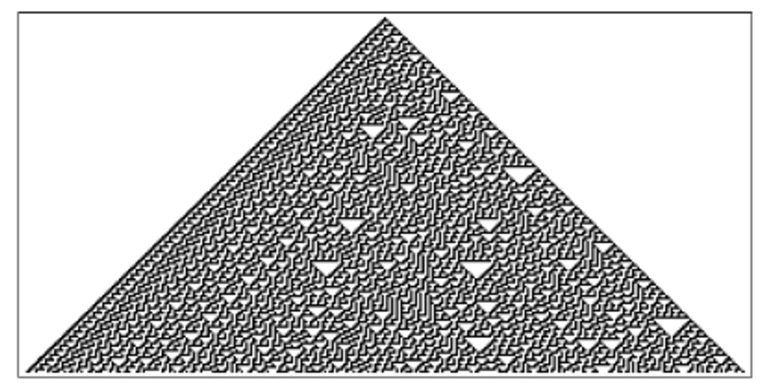
\includegraphics[scale=0.3]{figures/rule_30_cellular_automaton}}

\caption{The ``rule 30'' cellular automaton, which seems to be random, although
generated by simple rules. \label{fig:The-rule-30}}
\end{figure}

The recently-named field of ``executable biology'' \cite{fisher2007executable}
that focuses on the design of executable computer algorithms that
mimic biological phenomena \cite{fisher2007executable} can be viewed
as following the intuition of Stephen Wolfram to develop ``a new
kind of science''.

\part{Introduction}
\begin{quotation}
``Cellular automata are {[}...{]} idealizations of physical systems
in which space and time are discrete, and physical quantities take
on a finite set of discrete values.'' Stephen Wolfram \cite{wolfram1983statistical}
\end{quotation}
Cellular automata are based on simple rules but can display complex
behaviour. A cellular automaton consists of a regular lattice, with
a discrete variable at each site, and the state of a cellular automaton
is completely specified by the values of the variables at each site.
A cellular automaton evolves in discrete time steps and the value
of the variables at each site are only determined by the values of
the variables in its neighbourhood at the previous step. \cite{wolfram1983statistical}

\part{Scientific History}

The idea of cellular automata is attributed to Stanislas Ulaw and
John Von Neumann \cite{von1951general}, in the late 1940s-early 1950s
\cite{wolfram2002new}. Interestingly, John Von Neumann discovered
this idea while trying to develop an abstract model of self-reproduction
in biology. \cite{wolfram2002new}

The idea was not much investigated by science, but one example of
a cellular automaton did enter recreational computing in the early
1970s with James Conway's Game of Life, hat exhibit a range of complex
behavior. \cite{wolfram2002new}

\part{My Proposition}

My programme, written in C, can execute a cellular automata of variable
size, animal grazing rate and food\_growing rate through command line
arguments (see figure \vref{fig:Arguments-can-be}). It can display
different amounts of detail depending on whether the \textendash verbose
flag is activated (see figure \vref{fig:Comparison-between-the}).
The cellular automata resulting from runs of the programme are displayed
in the terminal (see figure \vref{fig:Comparison-between-the}).

The task of creating a cellular automata was modelled through an abstract
data structure representing the different objects that interact in
the cellular automaton (see figure \vref{fig:Abstract-class-(data})
and several functions (see figure \vref{fig:-Abstract-sequence}).
A run of the programme is depicted visually on figure \vref{fig:-Abstract-sequence}.

My code is available in the appendix. I have given variables meaningful
names so that the code can be read naturally. I have commented more
complicated parts of my code, as well as parts for which I had to
make a choice and I have described what functions perform on their
first line. My code is otherwise available on github at \url{https://github.com/MaxandreJ/Cellular_Automaton_Oxford_DTC}.
My code runs well.

\begin{figure}
\subfloat[A 5x5 grid has been created, following the first two arguments given
to the programme.]{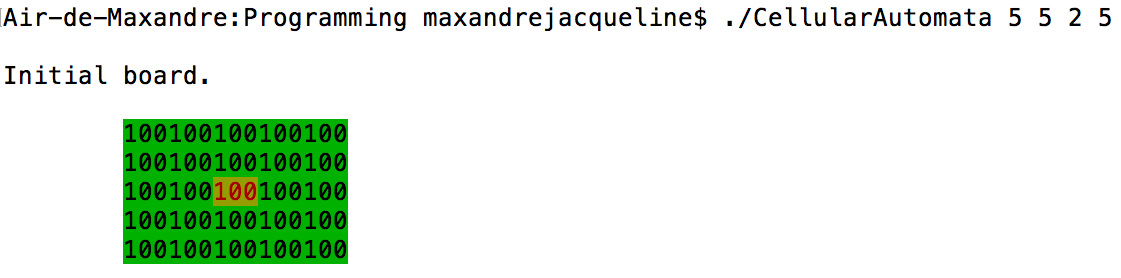
\includegraphics[scale=0.3]{figures/command_line_argument_5x5}

}

\subfloat[A 10x10 grid has been created, following the first two arguments given
to the programme.]{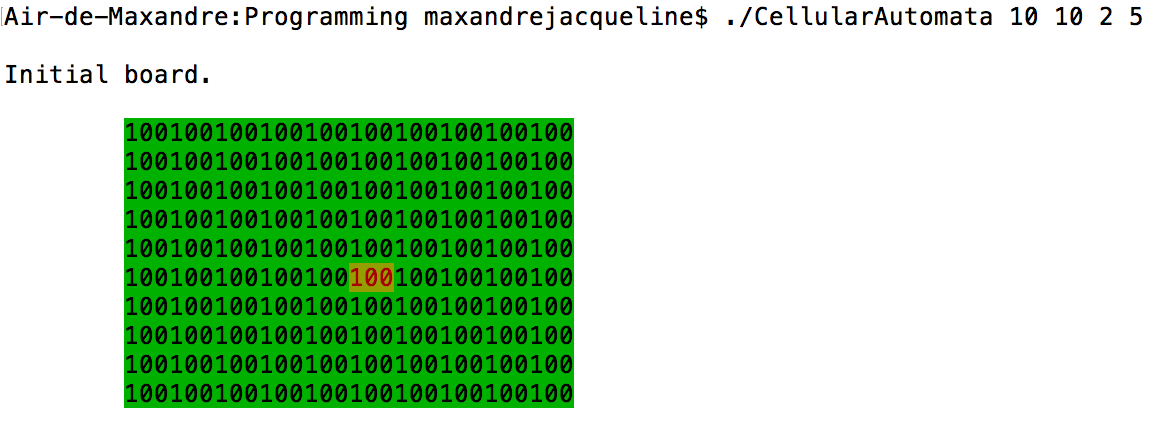
\includegraphics[scale=0.3]{figures/command_line_argument_10x10}

}

\caption[Arguments can be passed when calling the programme in the command
line.]{Arguments can be passed when calling the programme in the command
line. For example, you can make the grid small (sub-figure a), or
big (sub-figure b). Arguments are the following (in this order): number\_of\_rows,
number\_of\_columns, food\_growing\_rate, animal\_grazing\_rate, (-{}-verbose).
\label{fig:Arguments-can-be}}
\end{figure}

\begin{figure}

\subfloat[Default mode. Little information is given but one can see quickly
the overall changes.]{\centerline{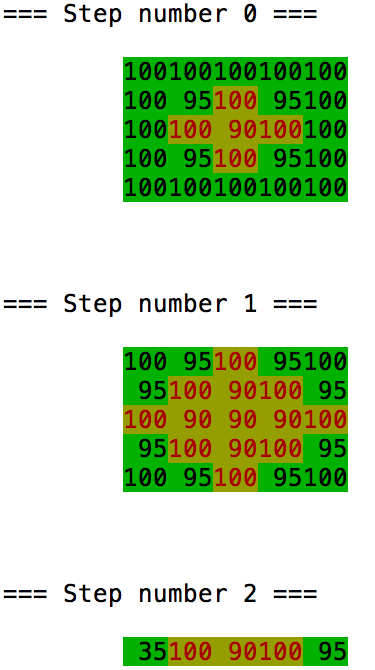
\includegraphics[scale=0.35]{figures/default_display}}

}

\subfloat[Verbose mode. Detailed information is given but it's hard to see the
overall changes.]{\centerline{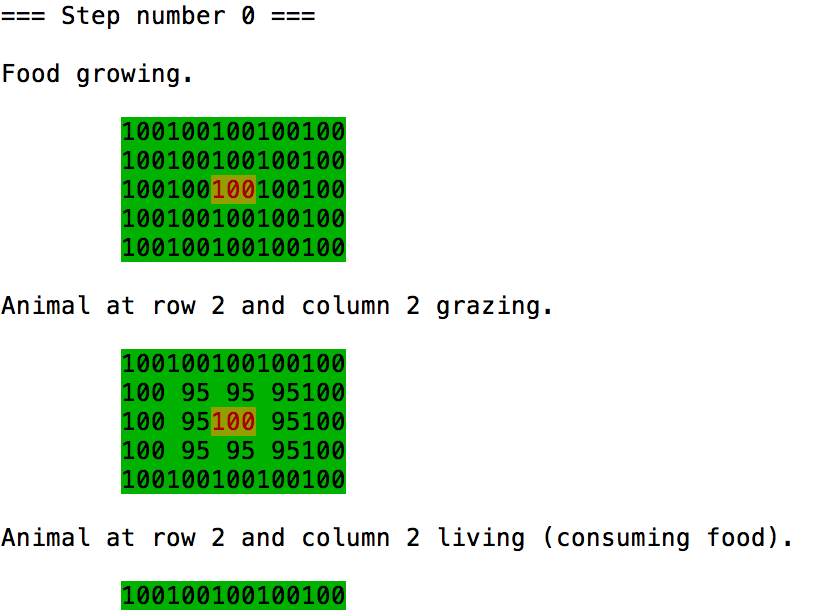
\includegraphics[scale=0.35]{figures/verbose_display}}

}\caption[Comparison between the default and the verbose mode.]{Comparison between the default (sub-figure a) and the verbose (sub-figure
b) mode. \protect \\
All displays were done on the terminal (also known as ``ASCII art'').
Green cells represent where food is, red cells: animals, yellow cells:
animals and food. If a cell is green, the number displayed in black
corresponds to the quantity of food available in the cell. If a cell
is red, the number displayed in black corresponds to the quantity
of food stored by the animal in that cell. If a cell is yellow the
number displayed in red corresponds to the quantity of food stored
by the animal in that cell (in that case, the quantity of food stored
in the cell is not displayed). \label{fig:Comparison-between-the}}

\end{figure}

\begin{figure}
\centerline{\includegraphics[scale=0.3]{\string"figures/abstract class diagram\string".png}}

\caption[Abstract class (data structure) diagram.]{Abstract class (data structure) diagram. I implemented it using type
definitions and structures in a header file. I did not try to implement
any methods because C is not an object-oriented language. \label{fig:Abstract-class-(data}}

\end{figure}

\begin{figure}
\centerline{\includegraphics[scale=0.2]{\string"figures/sequence diagram\string".png}}

\caption[Abstract sequence diagram.]{ Abstract sequence diagram. I implemented it separating each function
in a different file, and using a header file to link them together.
\label{fig:-Abstract-sequence}}
\end{figure}


\part*{Appendix: C Code}

\section*{Header}

\subsection*{CellularAutomata.h}

\begin{lstlisting}[language=C,numbers=left,breaklines=true]
#ifndef CELLULAR_AUTOMATA #define CELLULAR_AUTOMATA
//I need to give the prototype Board first, because functions that I use need //that type. typedef struct Board Board;
//Easy access to the position of an element //I use rows and columns instead of cartesian coordinates x and y because they are //confusing. A matrix doesn't have an orthonormal basis! typedef struct Position { int row; int column; } Position;
//Each food has a distinct quantity and growing_rata. In facts, I set it up //so that every Food has the same growing_rate, but my data structure allows it //to be different for each individual food. typedef struct Food { unsigned int quantity; int growing_rate; } Food;
Board grow_food(Board my_board);
//Animals can be present and dead. I don't use this distinction but it could be //used if one wanted to have zombie animals. //Using grazing_area_positions and breeding_area_positions allows easy access //to adjacent cells. typedef struct Animal { unsigned int present; unsigned int alive; unsigned int grazing_rate; unsigned int food_stored; unsigned int number_of_grazing_area_positions; unsigned int number_of_breeding_area_positions; int step_of_birth; Position grazing_area_positions[9]; Position breeding_area_positions[4]; Position position; } Animal;
//Animal constructor. Board construct_animal(Board my_board, int animal_position_row, int animal_position_column,   int animal_grazing_rate, int step_number); Board graze(Board my_board, Animal my_animal); Board live(Board my_board, Animal my_animal); //Each animal will have a "step of birth" based on the step_number that they are //born at. It allows for newly born animals not to breed instantly. Board breed(Board my_board, Animal my_animal, int animal_grazing_rate, int step_number);
typedef struct Cell { Position position; Animal animal; Food food; } Cell;
//The board, or in cellular automaton parlance "grid" has a cell_array_2D that //contains most of the data of this programme. The rest could be considered as //"metadata". struct Board { unsigned int number_of_rows; unsigned int number_of_columns; Cell** cell_array_2D; Position* food_positions; int amount_of_food; int number_of_animals; };
//The board constructor. Board construct_board(unsigned int number_of_rows, unsigned int number_of_columns, unsigned int food_growing_rate, unsigned int animal_grazing_rate); Board perform_step(Board my_board, int animal_grazing_rate, int step_number, int verbose_flag_chosen); void display_board(Board my_board);
#endif 
\end{lstlisting}


\section*{Main}

\subsection*{CellularAutomata.c}

\begin{lstlisting}[language=C,numbers=left,breaklines=true]
#include <stdio.h> #include <stdlib.h> #include <string.h> #include "CellularAutomata.h" /*    Cellular automata by Maxandre Jacqueline */
int main(int argc, char *argv[]) { 	Board my_board; 	unsigned int number_of_rows; 	unsigned int number_of_columns; 	unsigned int food_growing_rate; 	unsigned int animal_grazing_rate; 	int step_number = 0; 	char* verbose_flag; 	int verbose_flag_chosen;
	///Getting arguments from the command line
	if(argc == 5) 	{ 		number_of_rows = atoi(argv[1]); 		number_of_columns = atoi(argv[2]); 		food_growing_rate = atoi(argv[3]); 		animal_grazing_rate = atoi(argv[4]); 	} 	else if(argc == 6) 	{ 		number_of_rows = atoi(argv[1]); 		number_of_columns = atoi(argv[2]); 		food_growing_rate = atoi(argv[3]); 		animal_grazing_rate = atoi(argv[4]); 		verbose_flag = malloc(sizeof(char)*strlen(argv[5])); 		verbose_flag = argv[5]; 	} 	else 	{ 	printf("Wrong number of arguments. They should be given in the following order:\n" 	"number_of_rows number_of_columns food_growing_rate animal_grazing_rate (--verbose)\n"); 	//If the wrong number of argument is given, exit. 	return(1); 	} 	//Awkward, should've used a library for arg_parse 	if (argc == 6) 	verbose_flag_chosen = (strcmp(verbose_flag,"--verbose") == 0); 	else 	verbose_flag_chosen = 0;
	my_board = construct_board(number_of_rows, number_of_columns, food_growing_rate, animal_grazing_rate);
	printf("\nInitial board.\n"); 	display_board(my_board);
	///Iterating until stopped by the user (Ctrl-C) 	while(1) 	{ 		printf("\n=== Step number %d ===\n", step_number); 		my_board = perform_step(my_board, animal_grazing_rate, step_number, verbose_flag_chosen); 		//If verbose_flag_chosen, perform_step will do the displaying. Otherwise 		//it will be up to main. 		if (!verbose_flag_chosen) 		{ 			display_board(my_board); 		} 		//To pause the programme 		getchar(); 		step_number++; 	}
	///I remember to free the memory allocated in the heap. 	///Nevertheless, the code is not exception safe... 	///C doesn't seem very user-friendly for handling exceptions. 	///What a surprise. 	free(my_board.cell_array_2D); 	free(my_board.food_positions); 	free(verbose_flag); 	return 0; } 
\end{lstlisting}


\section*{Functions}

\subsection*{breed.c}

\begin{lstlisting}[language=C,numbers=left,breaklines=true]
#include <stdio.h> #include <stdlib.h> #include "../CellularAutomata.h"
Board breed(Board my_board, Animal my_animal, int animal_grazing_rate, int step_number) {   //An animal breeds in adjacent cells (at most 1 cell away, excluding diagonals)   //on the board.
  Cell my_bred_cell;   int number_position_breeding_area;   int my_bred_cell_row;   int my_bred_cell_column;
  if (my_animal.alive)   {     for (number_position_breeding_area=0;       number_position_breeding_area<my_animal.number_of_breeding_area_positions;       number_position_breeding_area++)     {       my_bred_cell_row = my_animal.breeding_area_positions[number_position_breeding_area].row;       my_bred_cell_column = my_animal.breeding_area_positions[number_position_breeding_area].column;
      my_bred_cell = my_board.cell_array_2D[my_bred_cell_row][my_bred_cell_column];
      //An animal can breed on a cell only if an animal is not already present       if (!my_bred_cell.animal.present)       {         my_board = construct_animal(my_board, my_bred_cell_row, my_bred_cell_column,           animal_grazing_rate, step_number);       }     }   }
  return my_board; } 
\end{lstlisting}


\subsection*{construct\_animal.c}

\begin{lstlisting}[language=C,numbers=left,breaklines=true]
#include <stdio.h> #include <stdlib.h> #include "../CellularAutomata.h"
Board construct_animal(Board my_board, int animal_position_row, int animal_position_column,   int animal_grazing_rate, int step_number) {   //Constructor for an animal. Returns a board with an added animal (so it is   //not exactly a constructor, but that'll do).
  Animal my_animal;   int row_offset;   int column_offset;   int breeding_position_counter = 0;   int grazing_position_counter = 0;   int position_within_borders;   int up_down_left_xor_right;
  Cell my_cell_with_animal;
  my_cell_with_animal = my_board.cell_array_2D[animal_position_row][animal_position_column];
  my_animal = my_cell_with_animal.animal;   my_animal.position.row = animal_position_row;   my_animal.position.column = animal_position_column;   my_animal.present = 1;   my_animal.alive = 1;   my_animal.grazing_rate = animal_grazing_rate;   //my_animal.food_stored is equivalent to its "health points" (HP).   my_animal.food_stored = 100;   my_animal.step_of_birth = step_number;
  //Definition of the positions of the grazing_area for my_animal   //Everywhere one unit away from my_animal, including diagonals   for (row_offset = -1 ;row_offset<=1;row_offset++)     {       for (column_offset = -1 ;column_offset<=1;column_offset++)         {           //Making sure we're not defining positions out of the board         position_within_borders = (           (animal_position_row + row_offset >= 0) &&         (animal_position_row + row_offset < my_board.number_of_rows) &&         (animal_position_column + column_offset >= 0) &&       (animal_position_column + column_offset < my_board.number_of_columns));
        if (position_within_borders)         {           my_animal.grazing_area_positions[grazing_position_counter].row = animal_position_row + row_offset;           my_animal.grazing_area_positions[grazing_position_counter].column = animal_position_column + column_offset;           grazing_position_counter++;         }         }     }     my_animal.number_of_grazing_area_positions = grazing_position_counter;
  //Definition of the positions of the breeding_area for my_animal   //Everywhere one unit away from my_animal, excluding diagonals   for (row_offset = -1 ;row_offset<=1;row_offset++)   {     for (column_offset = -1 ;column_offset<=1;column_offset++)       {         //Making sure we're not defining positions out of the board         position_within_borders = (           (animal_position_row + row_offset >= 0) &&           (animal_position_row + row_offset < my_board.number_of_rows) &&           (animal_position_column + column_offset >= 0) &&         (animal_position_column + column_offset < my_board.number_of_columns)         );         if (position_within_borders)         {           up_down_left_xor_right = ((row_offset == 0) || (column_offset == 0)) &&           (!((row_offset == 0) && (column_offset == 0)));           // An animal can only breed up xor down xor left xor right           if (up_down_left_xor_right)           {             my_animal.breeding_area_positions[breeding_position_counter].row = animal_position_row + row_offset;             my_animal.breeding_area_positions[breeding_position_counter].column = animal_position_column + column_offset;             breeding_position_counter++;           }         }       }   }   my_animal.number_of_breeding_area_positions = breeding_position_counter;   my_board.cell_array_2D[animal_position_row][animal_position_column].animal = my_animal;   my_board.number_of_animals += 1;
  return my_board; } 
\end{lstlisting}


\subsection*{construct\_board.c}

\begin{lstlisting}[language=C,numbers=left,breaklines=true]
#include "../CellularAutomata.h" #include <stdlib.h> #include <stdio.h>
Board construct_board(unsigned int number_of_rows, unsigned int number_of_columns, unsigned int food_growing_rate, unsigned int animal_grazing_rate) {   //Constructs the board, with the right size, animals and food.
	int row_number; 	int column_number; 	Cell my_cell; 	Board my_board; 	Animal my_animal; 	Food my_food; 	int animal_position_row; 	int animal_position_column; 	int food_position_counter = 0;   int step_number = -1;
	my_board.number_of_rows = number_of_rows; 	my_board.number_of_columns = number_of_columns;
	my_board.cell_array_2D = malloc(sizeof(Cell*)*my_board.number_of_rows);
  //In the present state, my_board.food_positions is useless.   //But potentially it could be used for defining that food is not present   //everywhere. 	my_board.food_positions = malloc(sizeof(Position)*(my_board.number_of_rows*my_board.number_of_columns));
	for (row_number=0;row_number<number_of_rows;row_number++) 	{ 		my_board.cell_array_2D[row_number]=malloc(sizeof(Cell)*my_board.number_of_columns); 		for (column_number=0;column_number<number_of_columns;column_number++) 		{ 			my_cell = my_board.cell_array_2D[row_number][column_number]; 			my_cell.position.row = row_number; 			my_cell.position.column = column_number;
			///Food set-up 			my_food = my_cell.food; 			my_food.quantity = 100;
			//Store the places where there's food in a different array 			my_board.food_positions[food_position_counter].row =  my_cell.position.row; 			my_board.food_positions[food_position_counter].column =  my_cell.position.column; 			food_position_counter++;
			my_food.growing_rate = food_growing_rate;
			///No animal except the one defined after the loop 			my_animal = my_cell.animal;
			my_animal.present = 0;
			my_cell.animal = my_animal; 			my_cell.food = my_food; 			my_board.cell_array_2D[row_number][column_number] = my_cell;
		} 	}
  //In the present state, my_board.amount_of_food is useless.   //see remark on my_board.food_positions   my_board.amount_of_food  = my_board.number_of_rows * my_board.number_of_columns;
	//I'm putting an animal in the centre of my board.   my_board.number_of_animals = 0; 	animal_position_row = number_of_rows / 2; 	animal_position_column = number_of_columns / 2;
  my_board = construct_animal(my_board, animal_position_row, animal_position_column,     animal_grazing_rate, step_number);
	return my_board;
} 
\end{lstlisting}


\subsection*{display\_board.c}

\begin{lstlisting}[language=C,numbers=left,breaklines=true]
#include "../CellularAutomata.h" #include <stdlib.h> #include <stdio.h>
Board construct_board(unsigned int number_of_rows, unsigned int number_of_columns, unsigned int food_growing_rate, unsigned int animal_grazing_rate) {   //Constructs the board, with the right size, animals and food.
	int row_number; 	int column_number; 	Cell my_cell; 	Board my_board; 	Animal my_animal; 	Food my_food; 	int animal_position_row; 	int animal_position_column; 	int food_position_counter = 0;   int step_number = -1;
	my_board.number_of_rows = number_of_rows; 	my_board.number_of_columns = number_of_columns;
	my_board.cell_array_2D = malloc(sizeof(Cell*)*my_board.number_of_rows);
  //In the present state, my_board.food_positions is useless.   //But potentially it could be used for defining that food is not present   //everywhere. 	my_board.food_positions = malloc(sizeof(Position)*(my_board.number_of_rows*my_board.number_of_columns));
	for (row_number=0;row_number<number_of_rows;row_number++) 	{ 		my_board.cell_array_2D[row_number]=malloc(sizeof(Cell)*my_board.number_of_columns); 		for (column_number=0;column_number<number_of_columns;column_number++) 		{ 			my_cell = my_board.cell_array_2D[row_number][column_number]; 			my_cell.position.row = row_number; 			my_cell.position.column = column_number;
			///Food set-up 			my_food = my_cell.food; 			my_food.quantity = 100;
			//Store the places where there's food in a different array 			my_board.food_positions[food_position_counter].row =  my_cell.position.row; 			my_board.food_positions[food_position_counter].column =  my_cell.position.column; 			food_position_counter++;
			my_food.growing_rate = food_growing_rate;
			///No animal except the one defined after the loop 			my_animal = my_cell.animal;
			my_animal.present = 0;
			my_cell.animal = my_animal; 			my_cell.food = my_food; 			my_board.cell_array_2D[row_number][column_number] = my_cell;
		} 	}
  //In the present state, my_board.amount_of_food is useless.   //see remark on my_board.food_positions   my_board.amount_of_food  = my_board.number_of_rows * my_board.number_of_columns;
	//I'm putting an animal in the centre of my board.   my_board.number_of_animals = 0; 	animal_position_row = number_of_rows / 2; 	animal_position_column = number_of_columns / 2;
  my_board = construct_animal(my_board, animal_position_row, animal_position_column,     animal_grazing_rate, step_number);
	return my_board;
} 
\end{lstlisting}


\subsection*{graze.c}

\begin{lstlisting}[language=C,numbers=left,breaklines=true]
#include <stdio.h> #include <stdlib.h> #include "../CellularAutomata.h"
Board graze(Board my_board, Animal my_animal) {   //An animal grazes (eats) in all adjacent cells (at most 1 cell away,   //including diagonals) on the board.
	Cell my_grazed_cell; 	int number_position_grazing_area; 	int my_grazed_cell_row; 	int my_grazed_cell_column;
	for(number_position_grazing_area=0;number_position_grazing_area<9;number_position_grazing_area++) 	{ 		my_grazed_cell_row = my_animal.grazing_area_positions[number_position_grazing_area].row; 		my_grazed_cell_column = my_animal.grazing_area_positions[number_position_grazing_area].column;
		my_grazed_cell = my_board.cell_array_2D[my_grazed_cell_row][my_grazed_cell_column];
    //If the grazed cell has enough food for the animal's grazing rate 		if(my_grazed_cell.food.quantity >= my_animal.grazing_rate) 		{ 		//Reducing the amount of food in the cell 		my_grazed_cell.food.quantity -= my_animal.grazing_rate; 			//Storing that food in the animal       //The amount of food stored by an animal can't exceed 100. 			if(my_animal.food_stored + my_animal.grazing_rate <= 100) 			my_animal.food_stored += my_animal.grazing_rate; 			else 			my_animal.food_stored = 100; 		} 		//If the grazed cell doesn't have enough food for the animal's grazing_rate 		else 		{       //Storing what's left food in the animal       //The amount of food stored by an animal can't exceed 100. 			if(my_animal.food_stored + my_grazed_cell.food.quantity <= 100) 			my_animal.food_stored += my_grazed_cell.food.quantity; 			else 			my_animal.food_stored = 100;
			my_grazed_cell.food.quantity = 0; 		}
		// I'm passing variables by value so I need to do lots of copying. 		// Passing by reference would be more memory efficient. 		my_board.cell_array_2D[my_grazed_cell_row][my_grazed_cell_column] = my_grazed_cell; 	} 	my_board.cell_array_2D[my_animal.position.row][my_animal.position.column].animal = my_animal;
	return(my_board); } 
\end{lstlisting}


\subsection*{grow\_food.c}

\begin{lstlisting}[language=C,numbers=left,breaklines=true]
#include <stdio.h> #include <stdlib.h> #include "../CellularAutomata.h"
Board grow_food(Board my_board) {   //Food grows everywhere there was ever food, in accordance to their growing_rate.   //By default, food is everywhere, so food grows everywhere.
int food_number; int my_food_row; int my_food_column;
for (food_number=0; food_number < my_board.amount_of_food; food_number++) 	{
	my_food_row = my_board.food_positions[food_number].row; 	my_food_column = my_board.food_positions[food_number].column;
  //The amount of food stored in a cell can't exceed 100. 	if(my_board.cell_array_2D[my_food_row][my_food_column].food.quantity <=     100 - my_board.cell_array_2D[my_food_row][my_food_column].food.growing_rate)
  //Every turn, food regrows by its growing_rate. 	my_board.cell_array_2D[my_food_row][my_food_column].food.quantity +=   my_board.cell_array_2D[my_food_row][my_food_column].food.growing_rate;
	else 	my_board.cell_array_2D[my_food_row][my_food_column].food.quantity = 100;
	}
return(my_board);
}; 
\end{lstlisting}


\subsection*{live.c}

\begin{lstlisting}[language=C,numbers=left,breaklines=true]
#include <stdio.h> #include <stdlib.h> #include "../CellularAutomata.h"
Board live(Board my_board, Animal my_animal) {   //An animal lives, which consumes energy by using up the food they have stored.
	if(my_animal.food_stored > 10)   { 	my_animal.food_stored -= 10;   }   //If the animal food consumption exceeds the amount of food he stored, it dies. 	else 	{ 	my_animal.present = 0; 	my_animal.alive = 0;   my_board.number_of_animals -= 1; 	}
	my_board.cell_array_2D[my_animal.position.row][my_animal.position.column].animal = my_animal;
	return(my_board); } 
\end{lstlisting}


\subsection*{perform\_step.c}

\begin{lstlisting}[language=C,numbers=left,breaklines=true]
#include <stdio.h> #include <stdlib.h> #include "../CellularAutomata.h"
Board perform_step(Board my_board, int animal_grazing_rate, int step_number, int verbose_flag_chosen) {   //A step of the game is performed.
	int number_of_animals; 	int amount_of_food;   int row_number;   int column_number;   int my_animal_eligible;   Cell my_cell; 	Animal my_animal; 	Position my_animal_position;
  my_board = grow_food(my_board);
  if (verbose_flag_chosen)   {   printf("\nFood growing.\n");   display_board(my_board);   }
  for (row_number=0;row_number<my_board.number_of_rows;row_number++)   {     for (column_number=0;column_number<my_board.number_of_columns;column_number++)     {     my_cell = my_board.cell_array_2D[row_number][column_number];     my_animal = my_cell.animal;
    //An animal can perform actions if it is present, alive, and born in a previous     //step.     my_animal_eligible = (my_animal.present && my_animal.alive       && (my_animal.step_of_birth < step_number));
    if (my_animal_eligible)     {   		my_board = graze(my_board, my_animal);       //Ugly, passing by reference my_animal would be better.       //But it can only be done by a pointer (not just by passing the reference, in C).       my_animal = my_board.cell_array_2D[my_animal.position.row][my_animal.position.column].animal;
      if (verbose_flag_chosen)       {       printf("Animal at row %d and column %d grazing.\n", my_animal.position.row,     my_animal.position.column);       display_board(my_board);       }
  		my_board = live(my_board, my_animal);       my_animal = my_board.cell_array_2D[my_animal.position.row][my_animal.position.column].animal;
      if (verbose_flag_chosen)       {       printf("Animal at row %d and column %d living (consuming food).\n", my_animal.position.row,     my_animal.position.column);       display_board(my_board);       }
      my_board = breed(my_board, my_animal, animal_grazing_rate, step_number);
      if (verbose_flag_chosen)       {       printf("Animal at row %d and column %d breeding.\n", my_animal.position.row,     my_animal.position.column);       display_board(my_board);       }
    }     } 	}
	return(my_board);
} 
\end{lstlisting}

\bibliographystyle{plain}
\bibliography{biblio_cellular_automaton}

\end{document}
